
\documentclass[10pt,twocolumn]{witseiepaper}
%
% All KJN's macros and goodies (some shameless borrowing from SPL)
\usepackage{KJN}
\usepackage[super]{nth}
\usepackage{subcaption}
\usepackage{listings}
\usepackage{amsmath}
\usepackage{epstopdf}
\usepackage{xcolor}
\usepackage{textcomp}
\usepackage{listings}
\usepackage{alltt}
\usepackage{matlab-prettifier}
\usepackage{graphicx}
\usepackage{changes}
\usepackage{makecell}
\usepackage{verbatim}
\usepackage{algorithm,algpseudocode}
\usepackage{balance}
\usepackage{pdfpages}
\usepackage{color} %red, green, blue, yellow, cyan, magenta, black, white
\definecolor{mygreen}{RGB}{28,172,0} % color values Red, Green, Blue
\definecolor{mylilas}{RGB}{170,55,241}
%\usepackage{flafter}

\lstset{language=Matlab, % Set colour for matlab code
	breaklines=true,%
	morekeywords={matlab2tikz},
	keywordstyle=\color{blue},%
	morekeywords=[2]{1}, keywordstyle=[2]{\color{black}},
	identifierstyle=\color{black},%
	stringstyle=\color{mylilas},
	commentstyle=\color{mygreen},%
	showstringspaces=false,%without this there will be a symbol in the places where there is a space
	numbers=left,%
	numberstyle={\tiny \color{black}},% size of the numbers
	numbersep=9pt, % this defines how far the numbers are from the text
	emph=[1]{for,end,break},emphstyle=[1]\color{red}, %some words to emphasise
	%emph=[2]{word1,word2}, emphstyle=[2]{style},    
}


%
% PDF Info
%
\ifpdf
\pdfinfo{
/Title (INSTRUCTIONS AND STYLE GUIDELINES FOR THE PREPARATION OF FINAL YEAR LABORATORY PROJECT PAPERS : 2005 VERSION)
/Author (Ken J Nixon)
/CreationDate (D:200309251200)
/ModDate (D:200510121530)
/Subject (ELEN417/455 Paper Format, 2005)
/Keywords (ELEN417, ELEN455, paper, instructions, style guidelines, laboratory project)
}
\fi

%%%%%%%%%%%%%%%%%%%%%%%%%%%%%%%%%%%%%%%%%%%%%%%%%%%%%%%%%%%%%%%%%%%%%%%%%%%%%%%
\begin{document}


\title{INSTRUCTIONS AND STYLE GUIDELINES FOR THE PREPARATION OF FINAL YEAR LABORATORY PROJECT PAPERS : 2005 VERSION}

\author{Sasha Berkiwitz () \& Lara Timm (704157)
\thanks{School of Electrical \& Information Engineering, University of the
Witwatersrand, Private Bag 3, 2050, Johannesburg, South Africa}
}


%%%%%%%%%%%%%%%%%%%%%%%%%%%%%%%%%%%%%%%%%%%%%%%%%%%%%%%%%%%%%%%%%%%%%%%%%%%%%%%
%
\abstract{}

\keywords{}


\maketitle
\thispagestyle{empty}
\pagestyle{plain}
\setcounter{page}{1}


%%%%%%%%%%%%%%%%%%%%%%%%%%%%%%%%%%%%%%%%%%%%%%%%%%%%%%%%%%%%%%%%%%%%%%%%%%%%%%%
\section{INTRODUCTION}

The report documents the design and implementation of a computer game, \textit{Shape Invaders}, created using C++14 and object-oriented programming. The basic game mechanics approximate those of the popular 1983 arcade game, Gyruss. 

Contained within the following sections are...

%%%%%%%%%%%%%%%%%%%%%%%%%%%%%%%%%%%%%%%%%%%%%%%%%%%%%%%%%%%%%%%%%%%%%%%%%%%%%%%
\section{PROBLEM DEFINITION}\label{probDef}


\subsection{Shape Invaders Game Play}

Shape Invaders, modelled on the arcade game Gyruss, is a C++14 developed computer game rendered using SFML~2.3.2. The game features a player character who moves around the circumference of a large circle. The player is capable of shooting at enemies, who spawn at the centre of the screen and travel outwards. The game is inhabited by a variety of enemies who are generated at random time intervals and at random angles. When colliding with an enemy or enemy bullet, the player looses a life. The player starts with five lives and the game ends when all of the players lives are depleted. Game speed increases with increasing time in game. As a result the objective of the game is to get the highest possible score rather than to destroy a limited number of enemies.

\subsection{Requirements}

The game contains the following basic functionality:

\begin{itemize}
	\item A player ship, player bullets, more than one enemy ship and enemy bullets exist.
	\item Enemy ships appear at the circle's centre, move radially outwards and eventually move off the screen. 
	\item The enemy ships fire bullets radially outwards towards the player. The player can fire bullets towards the centre of the circle.
	\item The game ends when the player is killed.
\end{itemize}

The game also contains the following features which enhance the game functionality:

\begin{itemize}
	\item The player begins the game with five lives. The player loses a life when colliding with another game object. Remaining lives are displayed in the bottom left hand corner of the screen.
	\item A scoring system is implemented. The player is awarded points for destroying other game objects. High scores are saved from one game to the next. The player's current score and the high score are displayed at the top of the screen.
	\item The game has additional game objects including asteroids, laser-generators and satellites.
	\item Asteroids travel radially from the circle's centre directly at the player. Asteroids cannot be destroyed.
	\item Laser generators appear in pairs at the circle's centre and laser force field is generated along an arc between them. If the player shoots either generator, the force field collapses.
	\item Satellites appear in groups of three in front of the player. They gyrate in small circles and shoot at the player. If all three satellites are shot, the player's gun is upgraded. Losing a life results in the player's gun being downgraded.
	
\end{itemize}


\subsection{Success Criteria}

To be deemed a success, the game should effectively implement the aforementioned functionality. This will result in game which runs smoothly, is easy to understand and is challenging. The game should be constructed using object-oriented programming, make use of good programming practises and should follow the separation of concern principle. 

\subsection{Constraints}

The final product must run on the Windows platform and be coded using the \textit{SFML 2.3.2} library. The game must display correctly on a screen with a maximum resolution of $1920 \times 1080$ pixels.

%%%%%%%%%%%%%%%%%%%%%%%%%%%%%%%%%%%%%%%%%%%%%%%%%%%%%%%%%%%%%%%%%%%%%%%%%%%%%%%
\section{CODE STRUCTURE AND IMPLEMENTATION}

On consideration of the design objectives in Section~\ref{probDef}, and in an attempt to code using good coding practises, the separation of layers principle was a pivotal design consideration. The remainder of this section describes the structure of the implemented code.

The code is separated into three distinct layers: the data layer, application logic layer and presentation layer. This was done in an attempt to implement the separation of concerns principle which will allow for decoupling of dependencies between classes. Communication between layers is carried out using object conversions, ensuring that only the necessary information is exposed to the other layers.

The data layer is handled by the \texttt{FileReader} class, application logic layer by the \texttt{Game} class and interface layer handled by the \texttt{Interface} class.

\subsection{Domain Model}

The game consists of various objects which move around the game area. These objects are identified as \textit{GameObjects} and are listed below:
\begin{itemize}
	\item Player
	\item Player Bullet
	\item Enemy
	\item Enemy Bullet
	\item Asteroid
	\item Laser Generator
	\item Arc Segment
	\item Satellite
\end{itemize}

All \textit{GameObjects} are required to handle collisions with all other objects, must be able to move and must be drawable. 
%A visual representation of the domain model hierarchy can be found in Figure~\ref{fig:ModelHierarchy}.


%\begin{figure}[h]
%	\centering
%	%\includegraphics[width=\columnwidth]{domainModel.png}
%	\caption{}
%	\raggedright
%	\label{fig:ModelHierarchy}
%\end{figure}

\subsection{Data Layer Class Structure}

This layer is responsible for the fetching and handling of data contained in files outside the Game executable. This data can then be provided to the game at runtime.

\subsubsection{FileReader Class}
~\\
~\\
This class functions as a simple file reader and writer. The class is responsible for reading in a previous high score from a text file, and in turn writing a new high score to the text file if the high score is beat in the current game. The high score data is thus obtained by the data layer and passed to the presentation layer, via the application logic layer, so that the high score can be rendered on the screen in game. This process ensures that \texttt{FileReader} does not have direct access to the interface layer.

\subsection{Logic Layer Class Structure}

The logic layer forms the largest component of the game. This layer is responsible for the handling of all objects in the game, managing all in-game operations and launching and managing the game loop which controls all dynamic activity and game functionality. The layer can be divided into two main subsections. The first, logic, which manages the game operations and the flow of the game, and second, the domain classes, which manage all game objects and their interactions. 

\subsubsection{Game Class}
~\\
~\\
This class is the most important class in the game as it controls all game logic. Responsibilities of \texttt{Game} include setting up all pre-game variables and requirements, instantiating all required game objects for the game and running the game loop. This loop interacts with the \texttt{Interface} by providing it with all of the information it needs to render the correct game state as well as the progression and updating of the game during play. The inverse relationship also exists. \texttt{Interface} provides \texttt{Game} with information regarding user inputs, allowing the game to be updated accordingly. 

Other responsibilities of \texttt{Game} include the initiation of object movements, keeping track of cooldowns, triggering new object instantiation when cooldowns expire, resetting cooldowns using randomly generated numbers and keeping track of the score and high score status. \texttt{Game} sets a new high score via the data layer's \texttt{FileReader} class. 


\subsubsection{GameObject Class}
~\\
~\\
 This class is the base class from which all game objects are inherited. \texttt{GameObject} contains the base parameters and functionality for all objects which have a position, can move, can collide with other objects and are drawable. Each derived \texttt{GameObject} thus has a position and physical attributes which enable the presentation layer to render the object as required by the game.
 
 In addition to an object's position, each \texttt{GameObject} has a hit radius which enables the \texttt{Game} class to detect collisions between objects and provide the \texttt{Interface} with the appropriate updated object information for rendering.
 
\subsubsection{Player Class}
~\\
~\\
This class represents the user controlled object in the game and inherits from the \texttt{GameObject} class. A \texttt{Player} object moves directly as a result of a keyboard input. This input is detected by the \texttt{Interface}, using SFML event polling, and is  subsequently converted into logic based events which are passed back to the logic layer for interpretation. The \texttt{Player} can move clockwise or anti-clockwise around a large circle. This object is also able to fire a \texttt{PlayerBullet} with a keyboard input detected by the interface. A \texttt{Player} object's life is reduced when it collides with any other \texttt{GameObject}. When the \texttt{Player's} life is reduced to zero, the game ends.

\subsubsection{PlayerBullet Class}
~\\
~\\
This class represents an object inherited from the \texttt{GameObject} class which is spawned at the current position of the \texttt{Player} and travels linearly towards the centre of the screen where it is deleted. A collision of a \texttt{PlayerBullet} with an \texttt{Enemy}, \texttt{LaserGenerator} or \texttt{Satellite} object results in both objects being destroyed. A collision of a \texttt{PlayerBullet} with a non-destroyable object (\texttt{Asteriod} and \texttt{ArcSegment}) results in only the bullet being destroyed.

Depending on the gun level of the \texttt{Player}, one to three \texttt{PlayerBullets} are fired by a single user input. The gun is upgraded when a \texttt{Satellite} array is destroyed and degraded when the \texttt{Player} loses a life.

\subsubsection{Enemy Class}
~\\
~\\
A class inherited from the \texttt{GameObject} class. This class represents an object which spawns at the centre of the screen and travels radially at a random trajectory angle towards the circle's circumference. A collision of an \texttt{Enemy} with the \texttt{Player} results on the \texttt{Enemy} being destroyed. There are an unlimited number of \texttt{Enemy} objects that can spawn throughout a game and these objects fire \texttt{Enemy Bullets} along their path vector towards the edge of the screen.

\subsubsection{EnemyBullet Class}
~\\
~\\
This class represents an automatically generated bullet, fired by an \texttt{Enemy} object, which travels along the same trajectory as its \texttt{Enemy}. \texttt{Enemy Bullets} inherit from the \texttt{GameObject} class. A collision of an \texttt{Enemy Bullet} with the \texttt{Player} results on the \texttt{Enemy} being destroyed.

\subsubsection{Asteroid Class}
~\\
~\\
This class represents non-destroyable objects which travel from the centre of the screen towards the \texttt{Player's} current position. This class is inherited from the \texttt{GameObject} class. 

\subsubsection{LaserGenerator Class}
~\\
~\\
This class is inherited from the \texttt{GameObject} class and represents an object which is instantiated in a pair and travels radially outwards. A pair of \texttt{LaserGenerators} is connected by a number of \texttt{ArcSegments} which travel in an arc between them. A collision of a \texttt{LaserGenerator} with the \texttt{Player} results in the destruction of the entire configuration. A collision of a \texttt{LaserGenerator} with a \texttt{PlayerBullet} results its destruction, as well as the destruction of all associated \texttt{ArcSegments}; namely the forcefield collapses.

\subsubsection{ArcSegment Class}
~\\
~\\
This class represents an object which forms an arc between two \texttt{LaserGenerators}, and is inherited from the \texttt{GameObject} class. A collision of an \texttt{ArcSegment} with the \texttt{Player} results in the destruction of the entire configuration.

\subsubsection{Satellite Class}
~\\
~\\
This class represents an object which spawns in an array of three directly in front of the \texttt{Player's} current position. \texttt{Satellites}, inherited from the \texttt{GameObject} class, gyrate in small circles and periodically fire bullets outwards.
A collision of a \texttt{Satellite} with a \texttt{PlayerBullet} results in its destruction.
The destruction of three associated \texttt{Satellites} results in an upgraded gun for the \texttt{Player}.

\subsection{Presentation Layer Class Structure}

This layer is responsible for polling of all user inputs and managing and rendering to the game window. The majority of presentation layer functionality is dependant of the \textit{SFML} library. This layer can be thought of as an interchangeable layer whereby any multimedia library could be used to replace it. SFML is used solely in the presentation layer allowing the application logic layer to function independently of it.

\subsubsection{Interface Class}
~\\
~\\
This class is responsible for polling user inputs and rendering of all objects to the SFML \textit{RenderWindow}. User inputs are communicated to the logic layer via a vector of logic layer events to which all polled input events are added. Additionally, object conversations allow for game objects, passed from the logic layer to the presentation layer, to be rendered correctly to the window. 

Other responsibilities of the \texttt{Interface} include rendering the \texttt{Player's} remaining number of lives, the current score and the high score to the window. The \texttt{Interface} also renders the game splashscreen and game-over screen depending on the current game state.

%%%%%%%%%%%%%%%%%%%%%%%%%%%%%%%%%%%%%%%%%%%%%%%%%%%%%%%%%%%%%%%%%%%%%%%%%%%%%%%
\section{IN-GAME BEHAVIOUR}

The game is managed by the \texttt{Game} class, more specifically by the game loop. This loop is described by the flow of operations seen in Figure~\ref{fig:flowDiagram}. 

\begin{figure}[h]
	\centering
	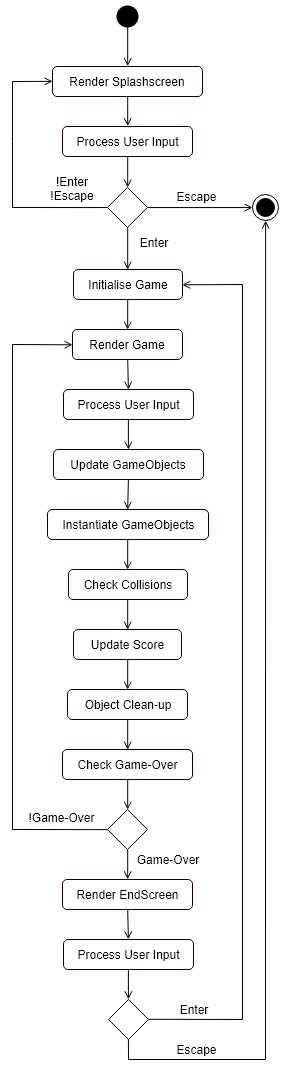
\includegraphics[width=\textwidth,height=0.9\textheight,keepaspectratio]{flowdiagram.png}
	\caption{Flow Diagram}
	\raggedright
	\label{fig:flowDiagram}
\end{figure}


The game begins by launching game-state one, the splashscreen. \texttt{Interface} then polls for user input; the enter key progresses the game to game-state two and escape closes the window and ends the game. Game-state two (the playing game state) loops continuously while the window is open and the \texttt{Player's} number of lives is greater than zero. 

The playing game-state proceeds in the following way. The \texttt{Interface} detects user input and the game is updated accordingly. New \texttt{GameObjects} are then created, collisions are detected, the score is updated and objects due for clean-up are deleted. If the \texttt{Player} object is deleted in clean-up, the end-game state is triggered and the game ends; otherwise the playing-state loops again.

\subsection{Game Input Polling}

An important aspect of the game design is separation of layers. Separating the presentation layer and the logic layer was an important 


\subsection{Collision Detection}



%%%%%%%%%%%%%%%%%%%%%%%%%%%%%%%%%%%%%%%%%%%%%%%%%%%%%%%%%%%%%%%%%%%%%%%%%%%%%%%
\section{CODE TESTING}

\subsection{Testing Environment}

\subsection{Data Layer Testing Structure}

\subsection{Application Layer Testing Structure}

%%%%%%%%%%%%%%%%%%%%%%%%%%%%%%%%%%%%%%%%%%%%%%%%%%%%%%%%%%%%%%%%%%%%%%%%%%%%%%%
\section{CRITICAL EVALUATION}

\subsection{Game Functionality}

\subsection{Code Structure and Implemented Design}

\subsection{Testing structure and Implementation}

%%%%%%%%%%%%%%%%%%%%%%%%%%%%%%%%%%%%%%%%%%%%%%%%%%%%%%%%%%%%%%%%%%%%%%%%%%%%%%%
\section{FUTURE IMPROVEMENTS}

\subsection{Game Functionality}

\subsection{Code Structure and Design}

\subsection{Testing structure}

%%%%%%%%%%%%%%%%%%%%%%%%%%%%%%%%%%%%%%%%%%%%%%%%%%%%%%%%%%%%%%%%%%%%%%%%%%%%%%%
\section{CONCLUSION}

%%%%%%%%%%%%%%%%%%%%%%%%%%%%%%%%%%%%%%%%%%%%%%%%%%%%%%%%%%%%%%%%%%%%%%%%%%%%%%%
%
%\nocite{*}
\bibliographystyle{witseie}
\bibliography{gameBib}

%{\tiny \vfill \hfill \today \hspace{5mm} witseie-paper-2003.\TeX}

\end{document}

" vim: ts=4
" vim: tw=78
" vim: autoindent
" vim: shiftwidth=4
